¿Qué es una fracción? Una fracción es una "parte" de un entero. Por ejemplo, si tengo la mitad de un chocolate, esa mitad es una fracción. Las fracciones se expresan de la siguiente manera:\\

\begin{equation}
    \notag
    \frac{3}{4} \longrightarrow \frac{Numerador}{Denominador}
\end{equation}


El Numerador es la cantidad de partes "que tengo" mientras que el Denominador es la cantidad de partes en la cual está partido el entero. En la figura siguiente se ejemplifica visualmente: 

\begin{figure}[H]
\centering
\fbox{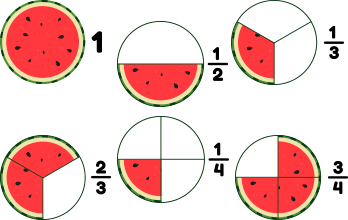
\includegraphics[width=0.5\linewidth]{images/fraccion.png}}
\label{1.0}
\end{figure}

Sin entrar en complicaciones, veamos simplemente las operaciones básicas de las fracciones: \\

\begin{itemize}
    \item Suma o resta con igual denominador: 
    \begin{equation}
        \notag
         \frac{a}{B} + \frac{b}{B} = \frac{a+ b}{B} \longrightarrow \frac{1}{2} + \frac{4}{2} = \frac{5}{2}
    \end{equation}
    \item Suma o resta con distinto denominador:
    \begin{equation}
        \notag
         \frac{a}{b} + \frac{c}{d} = \frac{a\cdot d + c\cdot b}{b\cdot d} \longrightarrow \frac{1}{2} + \frac{1}{3}=\frac{5}{6}
    \end{equation}
    \item Producto de fracciones: 
    \begin{equation}
        \notag
        \frac{a}{b}\cdot \frac{c}{d}=\frac{a\cdot c }{b \cdot d} \longrightarrow \frac{1}{2}\cdot \frac{3}{4}=\frac{3}{8}
    \end{equation}
    \item División de fracciones: 
    \begin{equation}
        \notag
            \frac{a}{b} : \frac{c}{d}=\frac{a\cdot d }{b \cdot c} \longrightarrow \frac{1}{2}\cdot \frac{3}{4}=\frac{4}{6}
    \end{equation}
\end{itemize}

Ejercicios:\\

\begin{enumerate}
\renewcommand{\labelenumi}{{\theenumi})}
\item $\frac{9}{3}-\frac{5}{6}$
\item $\frac{2}{5}\cdot \frac{12}{1}$
\item $\frac{4}{5}\cdot \frac{6}{1} : \frac{2}{11}$

\end{enumerate}